\documentclass{article}
\usepackage{graphicx}

\usepackage{arxiv}

\usepackage[utf8]{inputenc} % allow utf-8 input
\usepackage[T1]{fontenc}    % use 8-bit T1 fonts
\usepackage[colorlinks]{hyperref}       % hyperlinks
\usepackage{url}            % simple URL typesetting
\usepackage{booktabs}       % professional-quality tables
\usepackage{amsfonts,amsmath} % blackboard math symbols
\usepackage{nicefrac}       % compact symbols for 1/2, etc.
\usepackage{microtype}      % microtypography
\usepackage[bbgreekl]{mathbbol} % for blackboard \sigma
\usepackage{color}
\usepackage[square]{natbib}


\newcommand{\CC}{\mathbb C}
\renewcommand{\div}{\operatorname{div}}
\newcommand{\eq}[1]{\begin{equation}#1\end{equation}}
\newcommand{\II}{\mathbb I}
\newcommand{\jmp}[1]{[\![#1]\!]}
\newcommand{\nn}{\vc n}
\newcommand{\uu}{\vc u}
\newcommand{\vc}[1]{\boldsymbol{#1}}
\newcommand{\xx}{\vc x}
\newcommand{\todo}[1]{{\color{red}#1}}


\title{Stochastic modeling of EGS using continuum-fracture approach.}


\author{
  Jan Březina \\
  \And
  Pavel Exner \\
  \And
  Jan Stebel \\
  \And
  Martin Špetlík \\
  %% \AND
  %% Coauthor \\
  %% Affiliation \\
  %% Address \\
  %% \texttt{email} \\
  %% \And
  %% Coauthor \\
  %% Affiliation \\
  %% Address \\
  %% \texttt{email} \\
  %% \And
  %% Coauthor \\
  %% Affiliation \\
  %% Address \\
  %% \texttt{email} \\
}

\begin{document}
\maketitle

\begin{abstract}
Stochastic modeling of the hydraulic stimulation and long term operation of an enhanced geothermal system (EGS) is performed. The continuum-fracture approach is applied both for the stimulation model and for the operation model. Stochasticaly generated fractures and properties of the continuum are used in a simple hydro-mechanical model of the stimulation process. The resulting system of fractures with significant conductivity is used in the heat transfer model of the operation of the ground exchanger. The model is used to compute a single realization of key EGS properties: the output power and temperature. This complex sampling model is used within the Monte Carlo method predict probabilistic distribution for the EGS properties. The conceptual model and input data are loosely based on the geologic properties at the Litoměřice site in the Czech Republic.
\end{abstract}


% keywords can be removed
\keywords{First keyword \and Second keyword \and More}


\section{Introduction}
As the natural hydro thermal resources are sparse in the Czech Republic, the EGS (enhanced geothermal system) concept is subject of recent research focused on usage of the geothermal energy. According to the available geological data (\cite{Capova2013}), the Litoměřice site is the most attractive due to hot crystalline rock in relatively shallow depth (about 120 \textdegree C in 5km depth). This motivates development of the poroelasticity model within the Flow123d (\cite{flow123d}) simulator for the transport processes in the fractured porous media and its application in the study of uncertainty of the EGS properties caused by the fracture system.

The EGS approach depends on opening and reconnecting of the preexisting fracture network in the low permeable rock by the hydraulic stimulation and the temperature changes. Since the fracture network is a-priori unknown as well as spatial distribution of the key parameters, we should consider the operational parameters of the EGS as random variables. In order to predict their distribution the Monte Carlo method can be applied provided the forward model and the distribution of the input parameters. Considering the forward model, there are three main approaches are used for simulation of the transport processes in the fractured porous media, namely single continuum, discrete fracture networks and continuum-fracture approach.
The heterogeneous single continuum fully coupled THM model was used  in \cite{Watanabe2009} to study uncertainty in the output temperature. Usage of Monte Carlo method is natural in the DFN approach see e.g. \cite{Ezzedine2008}. 
We adopt the continuum-fracture approach which is much less common especially for significant technical difficulties. In \cite{Doonechaly2016} this approach was used for sensitivity analysis of the EGS operation, but only for the fixed fracture network. 

We consider simple two stage forward model. First, the hydraulic stimulation is described by the hydro-mechanical poroelasticity model combining discrete fractures and continuum. Linear elasticity is used, contact conditions and thermal effects, however they may be significant, are not considered. Based on the stimulation model the changed aperture and conductivity fields on the fractures are determined. Then the evolution of the temperature and the raw power output is simulated using the combined fracture-continuum approach for the thermo-hydraulic model as well. 
A realistic stochastic model for the distribution of the fractures is considered, other parameters are fixed as we want to study particularly the influence of fracture variability. 

\section{Conceptual model}
According to available geological data for the Litoměřice locality (see \cite{Capova2013}), the crystalline rock possibly consisting of granite, gneiss or mica schist 
% zula, rula, svor
is located in the depth
below 3 km. Two geological scenarios predict temperatures 140 C and 146 C respectively in the depth 5 km. We consider in our model two vertical wells in distance 200 m with opened part of the length 100 m located in the target depth of 5 km. The simulation domain is a box with dimensions $600\times600\times600$ m covering only the close neighbourhood of the stimulated domain. The wells are placed in the center. In order to reduce the complexity of the computational mesh, we
cut off cylinders of the radius 10 m at the wells positions and apply boundary conditions on their walls while avoiding very fine meshing at the wells scale.
This approximation is discussed in detail in Section \ref{}.
This simplified geometry is consistent with the simplification in the mathematical model as the precision of the model prediction is not of our interest in this work. We refer to the contribution paper \cite{Ralek} for the more EGS study for the Litoměřice locality.



\section{Hydro-mechanical model}
\label{sc:hm_model}
During the hydraulic stimulation the fluid is injected into both wells in order to open the preexisting fractures. This leads to increase in the aperture of fractures, which is then used in the production phase model described in the next section.
As the HM model of the bulk rock, we use the Biot poroelasticity equations:
\eq{\label{eq:biot} \partial_t(Sp + \alpha\div\uu) +\div\vc q = 0,\qquad -\div\bbsigma + \tilde\alpha\nabla h = 0. }
Here $\uu$ is the displacement [m], $p$ is the pressure head [m], $h=p+x_3$ is the piezo-metric head and the flux $\vc q$ [m.s -1] is given by the Darcy law
\eq{ \vc q = - k\nabla h}
with the hydraulic conductivity $k$. The coefficient $\tilde\alpha:=\alpha\varrho_l g$ where $\alpha$ is the Biot's effective stress parameter \cite{Biot1941},
$\rho_l$ is liquid density and $g$ is gravitational acceleration.
The stress tensor $\bbsigma$ [Pa] is given by the Hook's law
for the isotropic material:
\eq{ \bbsigma = \CC : \epsilon 
= (\lambda_M I\otimes I +2\mu_M I):\epsilon, \quad \epsilon = (\nabla \uu^T + \nabla \uu)/2}
with the Lamm\' e parameters: $\mu_M=E/(2(1+\nu))$ and $\lambda_M=E\nu/((1+\nu)(1-2\nu))$ [Pa].


The continuum-fracture approach consists in integration of the governing equations across the volume of a thin fracture effectively reducing its dimension to a 2d surface. This procedure was introduced by \cite{martin_modeling_2005} for the Darcy flow and extended for general advection-diffusion process in \cite{brezina_analysis_2015}. For the purpose of this work, the same approach was applied also to the equations of linear elasticity. We introduce the unit normal vector $\vc\nu$ to the fracture plane with arbitrary but fixed orientation.
For a general quantity $s$ that is defined on both faces of the fracture volume, we define the jump $\jmp{s}:=s^+-s^-$, where $s^\pm$ are the traces of $s$ on the faces. 
Then, integrating \eqref{eq:biot} across the fracture aperture results in the following system of equations:
\eq{\label{eq:biot_f}\left.\begin{aligned}
\delta\left(\partial_t\left(S_fp_f + \alpha_f\left(\div_\tau\uu_f+\tfrac1\delta\jmp{\uu}\cdot\vc\nu\right)\right) - k_f\Delta_\tau h_f\right) &= \jmp{F}, \\
\delta\left(-\div_\tau\CC_f(\nabla_\tau\uu_f+\tfrac1\delta\vc\nu\otimes\jmp{\uu}) + \tilde\alpha_f\nabla_\tau h_f\right) &= \jmp{\vc Q}.
\end{aligned}\right\} }
Here $p_f$ and $\uu_f$ denote the average pressure head and the average displacement on the fractures, respectively. The subscript $\tau$ indicates tangential operators on the fracture plane, $\otimes$ is the outer product and $\tilde\alpha_f:=\alpha_f\varrho_l g$.
The jumps $\jmp{F}=F^+-F^-$ and $\jmp{\vc Q}=\vc Q^+-\vc Q^-$ are the water sources and the forces, respectively,  that arise from the approximation of derivatives in the normal direction:
\eq{ 
\label{eq:fr_coupling}
\left.\begin{aligned}
F^\pm &:= \pm\frac2\delta k_f(h^\pm-h_f),\\
\vc Q^\pm &:= \pm\frac2\delta\CC_f(\nabla_\tau\uu^\pm + \vc\nu\otimes(\uu^\pm-\uu_f))\vc\nu. %\pm\frac2\delta\left(\mu_f(\uu^\pm-\uu_f)+(\mu_f+\lambda_f)((\uu^\pm-\uu_f)\cdot\vc\nu)\vc\nu\right) +\mu_f(\nabla_\tau\uu^\pm)^\top\vc\nu + \lambda_f(\div_\tau\uu^\pm)\vc\nu \pm\tilde\alpha_f p_f\vc\nu.
\end{aligned}\right\} 
}
System \eqref{eq:biot} and \eqref{eq:biot_f} is complemented by the boundary conditions for the bulk domain prescribed on the fracture faces:
\eq{ 
\label{eq:fr_coupling_bulk}
k\nabla h^\pm\cdot\vc\nu = F^\pm,\qquad \left(\CC(\nabla\uu^\pm) - \tilde\alpha h^\pm I\right)\vc\nu = \vc Q^\pm. 
}


For the sake of simplicity, we stimulate both wells simultaneously which results in very similar change of in the fracture aperture as if the wells were stimulated one by one.
Zero piezometric head and zero displacement are used as the initial conditions. The liquid is injected for 1 day under the stimulation pressure of 50 MPa (piezometric head $h_s=5e3$ m). This pressure is not applied directly on the surface of the well's cylinders, but through the Robin boundary condition with the transition parameter derived from the approximate analytical solution at the vicinity of the well.
The zero piezometric head is prescribed on the box sides, while the no flow condition is applied on the top and bottom face. Following boundary conditions were applied for the elasticity equation: zero displacement on the bottom of the box, zero normal displacement on the well's cylinders and zero traction elsewhere.

\section{Thermo-hydraulic model}
The TH model describes the heat transport in the EGS through the operation phase within 30 years after the hydraulic stimulation performed according to Section \ref{sc:hm_model}. In this scenario, we consider a steady Darcy flow: 
\eq{ \label{th_darcy}
    \div \vc q = 0, \quad \div  \vc q_f =  \jmp F,\quad
    \vc q_f = -\tilde\delta \tilde k_f \nabla h_f
}
for the bulk domain and fractures, respectively. Where $\tilde \delta$ is the fracture aperture updated according to the HM model.
The conductivity of the fractures is also adjusted according to the cubic law $\tilde k_f = k_f\tilde\delta_f^2 / \delta_f^2$
The communication between the fractures and the bulk rock is defined by the conditions \eqref{eq:fr_coupling} and \eqref{eq:fr_coupling_bulk}.

The heat transport model is sequentially coupled to the hydraulic model using computed Darcy flux $\vc q$ and $\vc q_f$. It assumes thermodynamic equilibrium between the liquid and the rock, the advection-diffusion equation for the bulk and fracture domain reads:
\eq{
\left.\begin{aligned}
&\partial_t\left(\tilde s T \right) + \div(\varrho_l c_l T \vc q) - \div(\lambda\nabla T) = 0,\\
&\partial_t\left(\delta \tilde s_f T_f \right) + \div(\varrho_l c_l T_f \vc q_f) - \div(\delta\lambda_f\nabla T_f) = \jmp{G}.
\end{aligned}\right\}
}
Here $T$ [$\circ$C] is the temperature, $\varrho_l$, $\varrho_s$ is the density, $c_l$, $c_s$ is the heat capacity.
\eq{
\tilde s = \vartheta \varrho_l c_l + (1-\vartheta)\varrho_s c_s,\quad 
\lambda= \vartheta \lambda_l + (1-\vartheta)\lambda_s
}
where $\theta$ is the porosity and $\lambda_l,\lambda_s$ is the thermal conductivity.

Similarly, to \eqref{eq:fr_coupling} we obtain the relation for the normal heat fluxes on the fracture faces:
\eq{ 
G^\pm &:= \pm\frac2\delta \lambda_f(T^\pm-T_f) + 
\varrho_l c_l F^\pm T_q,
}
where $T_q$ is equal to the bulk of fracture temperature as the normal Darcy flux $F^\pm$ is positive or negative, respectively. The system is completed by the bulk boundary conditions:
\eq{ 
- (\rho_l c_l \vc q T_q - \lambda\nabla T^\pm)\cdot\vc\nu = G^\pm.
}

The liquid is continuously injected into the left well under the injection pressure 0.5 MPa ($h_i = 50$ m) and pumped out to the level of the EGS 
($h_o = -5000$ m). No flux condition is used on the outer boundary. 
The injecting temperature is set to $15\ ^\circ$C, the natural convection 
heat flux is prescribed on the production well. The initial temperature field is considered on the outer boundary, which is given by 
 $10\ ^\circ$C at the Earth surface and the geothermal gradient $30\ ^\circ$C.km${}^{-1}$.

%We use the following system of heat equation and steady-state Darcy flow with coupling terms connecting the rock to the fractures:

% \subsection{Conductivity dependent on displacement}
% \textcolor{red}{PE: If not longer, move it directly to the description of flow above.}
% We consider that after releasing the fracking pressure the displacement of larger fractures persists. So the change in new porosity is
% \[
% \phi = \phi_0 + \alpha\div \vc u
% \]
% where $\phi_0$ is the porosity before deformation, c.f. time term in \eqref{eq:biot}. 
% Using the Carman-Kozeny relation \cite{Kaviany1999}, 
% % \[
% %     k = \tilde{k}\frac{\phi^3}{(1-\phi)^2}
% % \]
% we can derive formula for the updated conductivity:
% \[
%     K = K_0\left(\frac{\phi}{\phi_0}\right)^3 \left(\frac{1-\phi_0}{1-\phi}\right)^2.
% \]



\section{Geology and Model Parameters}

Most of the parameters used for computation are gathered in Table \ref{tab:params}.
The mechanical properties of granitic rocks have been investigated e.g. in \cite{Ljunggren1985}, where the measured Young modulus $E$ varies around 50 GPa and Poisson's ratio $\nu$ is around 0.25. The Biot coefficient for different rocks is hard to obtain, we use the value $\alpha=0.6$ inspired by \cite{Selvadurai2019}, where $\alpha$ for Grimsel granite varies between 0.46 to 0.72.
The reported values of the drained compressibility $\beta$ of several types of granite and orthogneiss are approx. $20\times 10^{-13}$ cm${}^2$.dyne${}^{-1}$ = $2\times10^{-11}$ Pa${}^{-1}$ \cite{Zisman1933}.
As far as porosity $\vartheta$ is concerned, \cite{intera} reports values between 0.001 and 0.01 for metamorphic crystalline rocks, we shall consider the value 0.005.
We assume the standard value of gravitational acceleration $g=9.81$ m.s${}^{-2}$.
%Here and in what follows, subscript ``l'' indicates quantities associated to the liquid.
%Similarly, subscript ``f'' will denote quantities for the fractures.
Storativity $S$ is calculated from water compressibility $\beta_l=5\times 10^{-10}$ Pa${}^{-1}$ and porosity following (\cite{Brace1968}, \cite{intera}):
\[ S = \varrho_l g(\beta + \vartheta\beta_l) \approx 2\times 10^{-7} \mbox{ m}^{-1}. \]


The values of physical parameters in the fractured zone are mostly unknown, hence the following values are only approximate.
The aperture of the fractures is considered constant in the input of the HM model according to \cite{Honza-clanek o laborratornich mikropuklinach??}.
After the process of the hydraulic fractioning, the aperture and hydraulic conductivity are adjusted according to the displacement results in TH model in \eqref{th_darcy}.
The hydraulic conductivity $k$ in the bulk rock is set similarly to \cite{Sperl2008} and \cite{Doonechaly2016}, where they also consider DFN and surrounding rock.
Additionally we assume that the hydraulic fractioning impacts also the smaller fractures not included in our DFN,
so we increase $k=10^{-8}$ of the bulk rock.


The hydraulic conductivity of fractures dominates than the one of intact rock by several orders of magnitude, we consider $k_f=10^{-3}$ m.s${}^{-1}$
On the other hand, the elastic modulus of fracture is assumed much smaller, we take $E_f=50$ Pa.
The porosity is taken one order higher that in the rock, i.e. we consider $\vartheta_f=0.05$.
We assume the same compressibility $\beta_f=\beta$, which gives approximately the same value of storativity $S_f\approx S$.

\begin{table}
\centering
\begin{tabular}{|l|c|c|c|}
\hline
 & rock & fractures & liquid\\\hline
Young modulus $E$ [Pa] & $50\times10^9$ & 50 & --- \\
Poisson's ratio $\nu$ [--] & 0.25 & 0.25 & --- \\
Biot's coefficient $\alpha$ [--] & 0.6 & 0.6 & --- \\
\hline
Density $\varrho$ [kg.m${}^{-3}$] & 2700 & 2700 & 1000 \\
Porosity $\vartheta$ [--] & $5\times10^{-3}$ & $0.8$ & --- \\
Compressibility $\beta$ [Pa${}^{-1}$] & $2\times10^{-11}$ & $2\times10^{-11}$ & $5\times10^{-10}$ \\
Storativity $S$ [m${}^{-1}$] & $2\times10^{-7}$ & $2\times10^{-7}$ & --- \\
Aperture $\delta$ [m] & --- & *$5\times10^{-5}$ & --- \\
Hydraulic conductivity $k$ [m.s${}^{-1}$] & *$10^{-9}$ & *$2.5\times10^{-3}$ & ---\\
\hline
Heat capacity $c$ [J.kg${}^{-1}$.K${}^{-1}$] & 790 & 790 & 4000 \\
Thermal conductivity $\lambda$ [W.m${}^{-1}$.K${}^{-1}$] & 2.5 & 2.5 & 0.5 \\
\hline
\end{tabular}
\caption{Physical parameters of rock, fractures and water, used in the model. \\ *) these values hold for HM model.}
\label{tab:params}
\end{table}

%Papers about effective properties of fractured porous media: \cite{Snow1969}, \cite{Bonnet2001}, \cite{Olson2003}



%\subsection{Parameters of EGS site and model geometry}

%Number of wells: 2 \\
%Depth: 5 km \\
%Distance: 200 m \\
%Well radius: $\rho = 15$ cm \\
%Length of open part of wells: $L=60$ m \\

% Pressure difference / water flux: 60 l/s


%In our model, we consider pair of vertical wells with the radius $\rho=0.15$ m in the distance $D=200$ m. The open part of the length $L=60$ m is in the depth $5000$ m. The cube $600 \times 600 \times 600$ m around the open parts is considered as the computational domain.

%{\bf The test geometry:} The wells are connected by three fractures, two of them intersecting the cylinders and one intersecting the first two fractures.



\subsection{Analytical models in the vicinity of the well}
We assume the well radii be $\rho = 15$ cm which is difficult to capture in the computational mesh.
In order to keep the mesh size treatable, we cut out of the computational domain two cylinders around the open well parts with a larger radius $R=10$ m.
On the surface of these cylinders we consider the Robin type boundary condition for the piezometric head:
%
\eq{\label{eq:H_robin} k\nabla h\cdot\nn = \sigma(H_w-h), }
%
where $\nn$ is the unit normal vector pointing to the centre of the well and $H_w$ is the piezometric head in the well.
% We assume the constant conductivity $k$ in the vicinity of well.
The parameter $\sigma$ is determined from the analytical radially symmetric solution
of the steady Darcy flow problem with a point source:
\[
    \hat h(r) = -\alpha \log (r) + \beta,
\]
where $r$ is the distance from the well and $\alpha$, $\beta$ are arbitrary constants such that $\hat h(\rho)=H_w$ holds.
First, the flux from the well into the domain through the surface $C_\rho$ of the cylinder with radius $\rho$ and length $L$ is
%  
\eq{\label{eq:Q_rho}    Q_\rho := -\int_{C_\rho} k\nabla h\cdot\nn = -2\pi \rho L k \hat h'(\rho) = 2\pi L k \alpha. }
%
% where we have used the Darcy law with the conductivity $k$.
%Now we use the analytical solution to fit the Robin type boundary condition:
Next, the flux at the distance $R$ can be expressed from \eqref{eq:H_robin} as follows:
%
\eq{\label{eq:Q_R}   Q_R = 2\pi R L \sigma (\hat h(\rho) - \hat h(R)) = 2\pi R L \sigma \alpha \log(R/\rho).}
%
%which combined with previous equality determines $\sigma$ as:
Finally, since $Q_\rho=Q_R$, we obtain from \eqref{eq:Q_rho} and \eqref{eq:Q_R}:
\eq{ \label{eq:sigma} \sigma = \frac{k}{R\log(R/\rho)}. }
In the simulations we shall use the hydraulic conductivity of the fractures in \eqref{eq:sigma} as the fractures have major influence on the flow in the vicinity of wells.

Since the heat transfer is dominated by the convection in the vicinity of the wells, the temperature in the well is transported to the surface of the cut-off cylinders or vice verse in the time $t_0 = R/q$ which for the observed volume fluxes $Q\sim 1$ l/s is about $100$ days. This is negligible with respect to the total lifetime of the heat exchanger, hence in the simulation of heat we shall use Dirichlet boundary condition for the temperature.

\subsection{Stochastic description of the fractures}
The fracture stochastic model consists of the Fisher's distribution for the fracture orientation, the power law for the fracture size, Poisson process for the number of fractures and uniform distribution for the fracture centers. The square fractures are considers with the side $r/2$. 
The von Mises-Fischer distribution \cite{Fisher1993} is used to describe orientation of single family of fractures with given mean normal vector $\vc a$ and the concentration parameter $\kappa$. The distribution is radially symmetric around $\vc a$ with the density function for the angle $\theta$ between $\vc a$ and fracture normal:
\[
 f(\theta) = c_\theta \exp(\kappa \cos(\theta)) \sin(\theta),
 \quad
 c_\theta = \frac{\kappa}{2\pi(\exp(\kappa) - \exp(-\kappa)}.
\] 
The power law distribution is considered for the fracture size $r$.
This kind of distribution is scale invariant, which is the key property of the natural fracture networks, see \cite{Bonnet2001} for detailed discussion. In practice the scale invariance holds only on some range of scales, leading to the truncated power law with the density:
\begin{equation}
    \label{eq:pow_law}
    f(r) = c_r r^{-(\gamma+1)},\quad 
    \frac{1}{c_r}=\int_{r_0}^{r_1} r^{-(\gamma+1)} dr = 
    \frac{r_0^{-\gamma} - r_1^{-\gamma}}{\gamma},
\end{equation}
for $r \in [r_0, r_1]$. 
For the given scale range, the number of fractures in unit volume is described by the Poison process with the intensity $\lambda=P_{30}[r_0, r_2]$ describing the mean number of fractures in the unit volume. The measurable parameter is the related mean total area per unit volume 
\[
P_{32} =
   \int_{r_0}^{r_1} r^2 f(r) dr =
    P_{30} \frac{\gamma}{2-\gamma}    \frac{r_0^{2-\gamma} - r_1^{2-\gamma}}
    {r_0^{-\gamma} - r_1^{-\gamma}}.
\]
In order to obtain fracture sets of the size tractable by our simulation tools, we represent explicitly only the fractures in the scale range $[r_2, r_3]$ while the scales $[r_0, r_1]$ are treated as equivalent porous media. The upper bound $r_3$ is set to the diameter of the simulation domain and upper scales are omitted. The lower bound is determined by desired mean intensity $P_{30}[r_2, r_3]$ through the relation:
\eq{
    \label{eq:pl_rescale}
    \frac{P_{30}[r_2, r_3]}{P_{30}[r_0, r_1]} 
    =
    \frac{r_2^{-\gamma} - r_3^{-\gamma}}
    {r_0^{-\gamma} - r_1^{-\gamma}}.
}
Positions of the fracture centers are sampled uniformly over the smaller box around the wells with dimensions $(300, 150, 150)$. 

Since no fracture statistics data for the target locality are available, we use data for the Forsmark site in Sweden
(\cite{Follin}) with a crystalline bedrock. Parameters of the distributions for five families of the fractures are summarized in Table.
\todo{JB: copy table from other word report}.

caption: Used stochastic parameters of the five fracture families. Parameters of the distributions of the fracture orientation, size and intensity.

% \subsection{Effective properties of the fractured porous media}
% Assuming the cubic law for the permeability of fracture and fracture independency (over simplification) the effective permeability tensor of the grid of parallel infinite fractures of the aperture $b$ and distance $D$
% is (\cite{Snow1969}):
% \[
%     K(b) = \frac{1}{12} \frac{b^3}{D} (I - \vc{n} \otimes \vc{n}) 
% \]
% Assuming superposition of fracture grids of different orientations, we can integrate over the $\vc n$ obtaining the factor $2/3$.  Further, assuming simplest linear relationship between the aperture and fracture size (\cite{Klimczak2010}) with a factor $\alpha$, we obtain:
% \begin{equation}
%     \label{eq:iso_perm}
%     k(b) = \frac{2}{3}\frac{1}{12} \frac{\alpha^3r^3}{D}
% \end{equation}
% for the isotropic permeability $k$. According to the power law \eqref{eq:power_law} distribution of the fracture sizes, there are
% \begin{equation}
%     \label{eq:n_frac}
%     N \sim f(r)dr
% \end{equation}
% fractures in the unit volume, with $r\in [r, r+dr]$. We can imagine to arrange these randomly spread fractures into a grid of unit squares with distance $D$, there are $1/Dr^2$ these tiles per unit volume. Comparing to \eqref{eq:n_frac}, we obtain
% \[
%     \frac{1}{D} \sim c_r r^{(1-\gamma)}
% \]
% substituting into \eqref{eq:iso_perm} and integrating over $[r_0, r_2]$,
% we obtain
% \[
%     k[r_0, r_2] \sim \frac{c_r}{18} \alpha^3 \frac{r_2^{(5-\gamma)} - r_0^{(5-\gamma)}}{5-\gamma}
% \]


\section{Numerical results}
The model described above was used to sample the production temperature and the heat power for the years 1 to 30. Single execution of the forward model consists of:
\begin{enumerate}
    \item drawing a fracture set sample according to Section 5.2
    \item create the geometry with fracture intersections and generate the mesh using own code and \cite{GMSH} meshing tool
    \item perform custom mesh healing algorithm to improve mesh quality
    \item execute Flow123d for the the HM model
    \item compute the modified aperture and conductivity for the fractures
    \item execute Flow123d for the TH model with opened fractures
    \item execute Flow123d for the TH model with unmodified fractures
\end{enumerate}
An example of a single realization of the fracture network is in Figure ...
confinement of the fracture centers to a box around the wells is clearly visible, we obtain pretty good intersection with the well cylinders but the fracture network typically does not create a connect path between the wells. Due to technical reasons, we used the expected number of fractures 100 and set $r_2$ accordingly using \eqref{eq:pl_rescale}, the domain diameter was used for the upper fracture size limit $r_3=600$. We do not expect significantly better connectivity of the network for larger number of fractures because due to the nature of the power law this only adds more smaller fractures. Temperature distribution on the fractures and on the vertical cut of the domain for the year 5 can be seen in Figures X and Y.
The influence of the fractures on the heat transfer in the bulk domain is clearly visible.

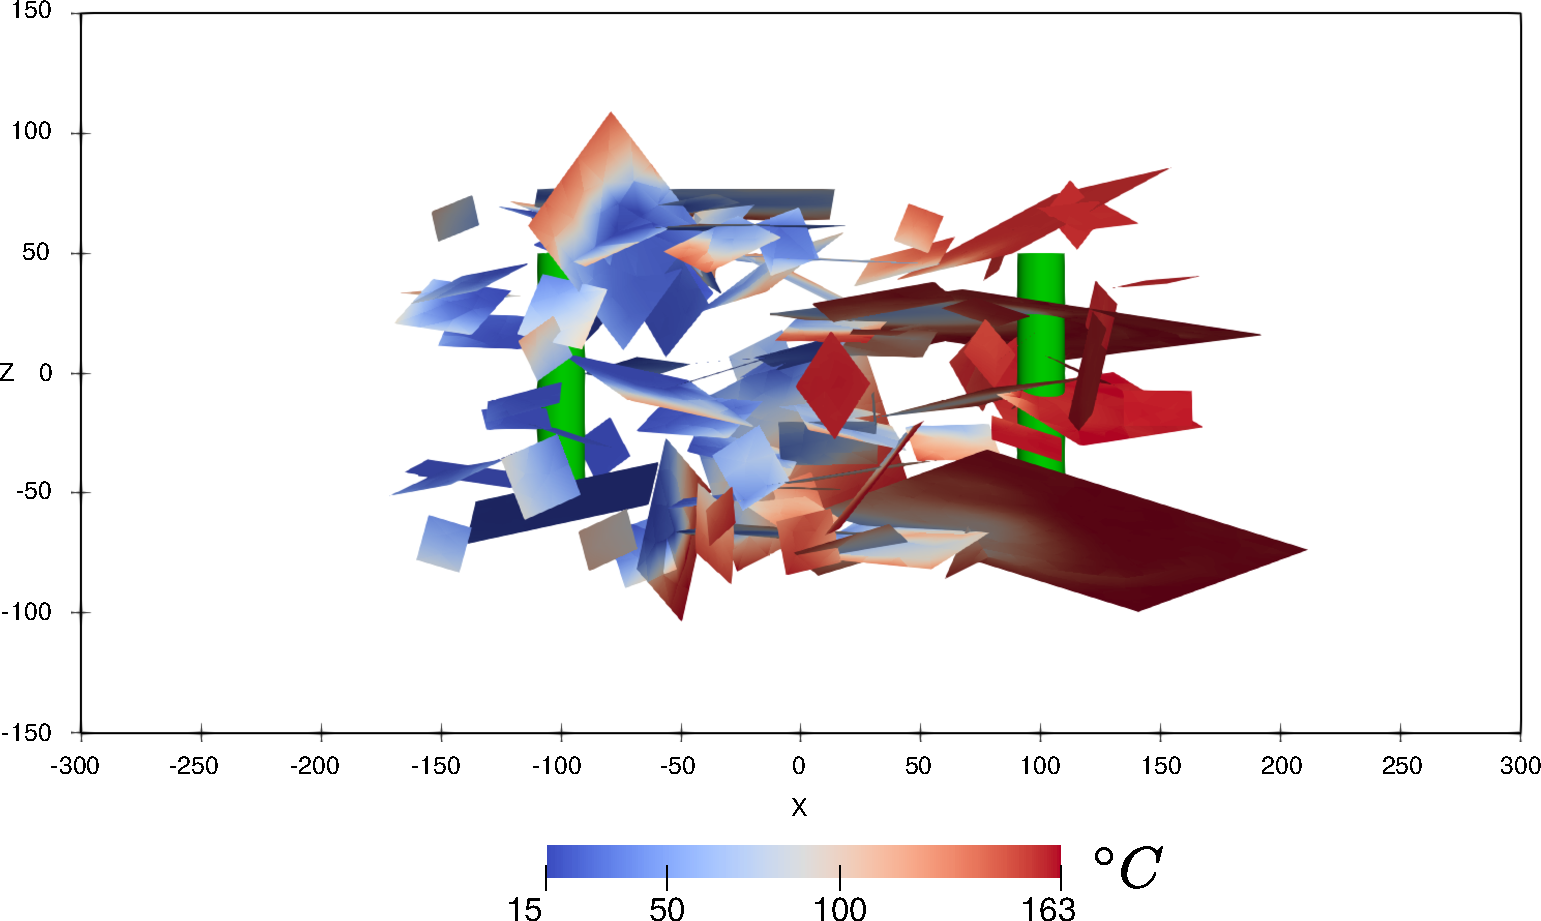
\includegraphics[width=\textwidth]{sample_6_bulk_t5_fr_final.pdf}
caption:
A fracture set sample with distribution of the temperature in the year 5 of the operation with the stimulated fractures.
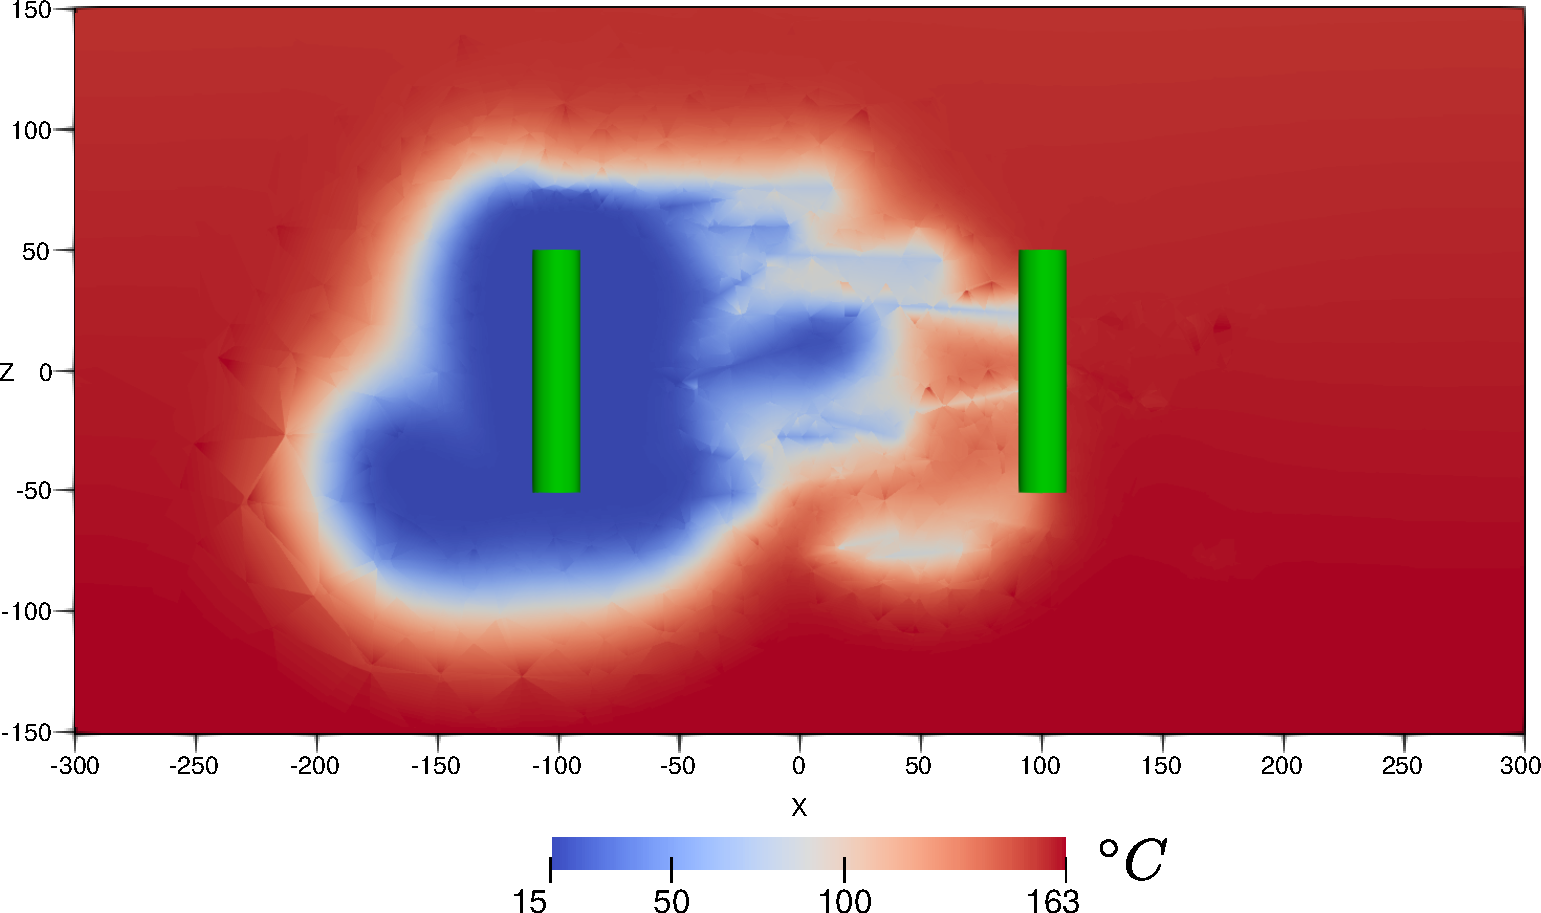
\includegraphics[width=\textwidth]{sample_6_bulk_t5_final.pdf}
caption:
Distribution of the temperature on the bulk domain in the year 5 for a single sample.


Total number of 1000 executions of the complete forward model was performed using a parallel cluster. These models have used a precomputed set of good meshes that were selected from about 2000 independent fracture sets.
Further about 100 samples were rejected because of the extremely bad temperatures caused by the instability of the used numerical method for some extremely heterogeneous cases of the modified conductivity of the fractures.
Remaining samples were used to estimate the mean and the standard deviance for the output temperature and the output power. Evolution of the mean and standard deviance is plotted in Figure ...
The histograms for the selected times 1, 15 and 30 is in the Figure ...
Absolute values especially for the power may not be realistic, but the important observation is the relation between the standard deviation and the gap between the stimulated and the reference case. As can bee seen from the histograms the distribution  for the power is close normal just slightly skewed for the initial times. Thus the standard variance corresponds to about 70\% of samples, say otherwise doing the stimulation
there is a 15\% chance you get the power below the plotted std band, which is not very small probability and the value is already pretty close to the reference non-stimulated case.

\begin{figure}
\includegraphics[width=0.5\textwidth]{mlmc_random_frac/output_scenarios/ power_comparison.pdf}
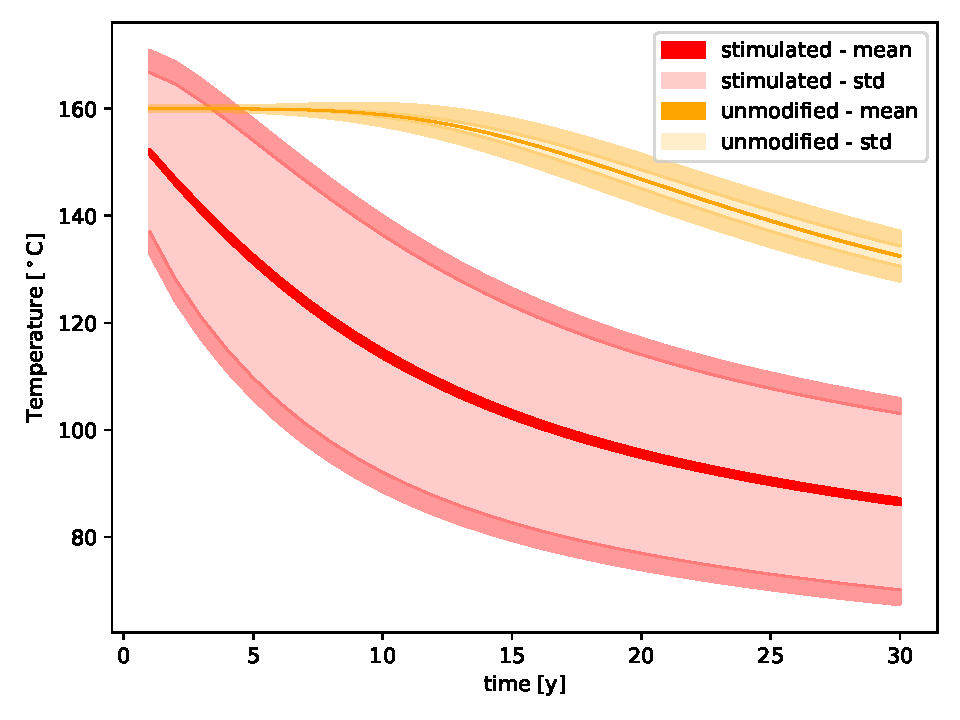
\includegraphics[width=0.5\textwidth]{temp_comparison.pdf}
\caption{Evolution of the estimated mean output temperature and the output power for the stimulated and unmodified fracture network. The band width is the error of estimation the wide transparent band is the estimate of the standard variance due to the fracture dispersion again with outer band marking the error of the estimation.}
\end{figure}

\begin{figure}
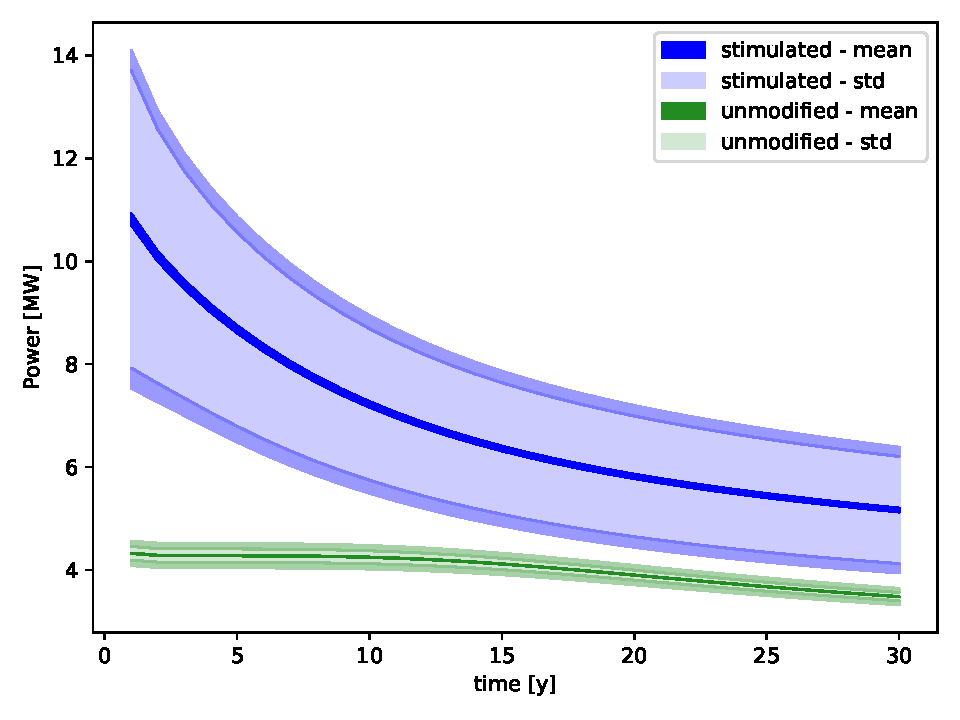
\includegraphics[width=0.5\textwidth]{power_comparison.pdf}
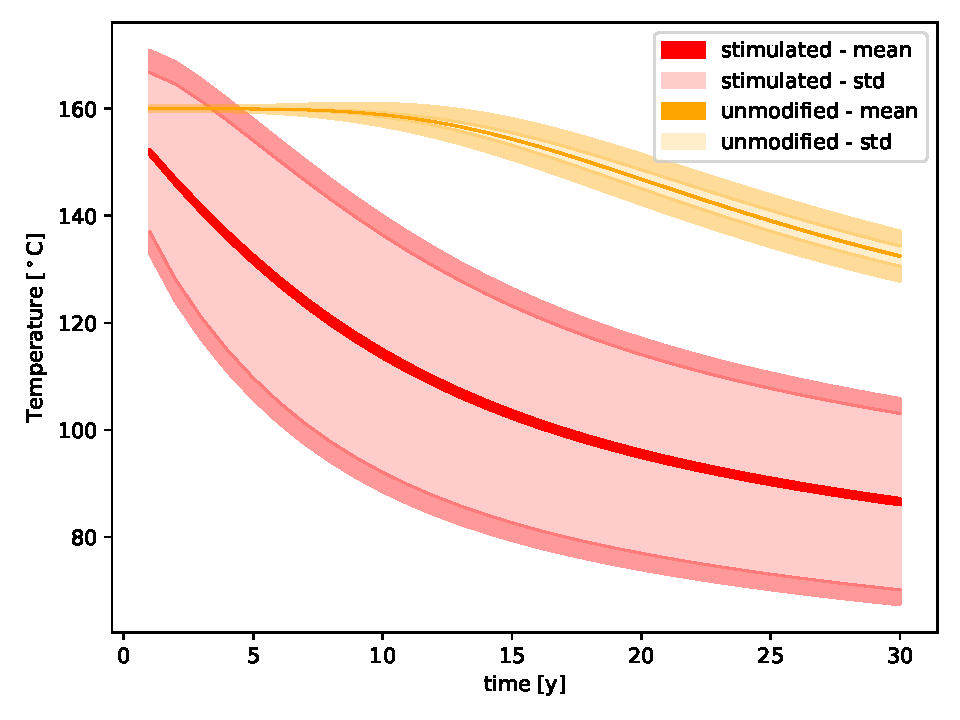
\includegraphics[width=0.5\textwidth]{temp_comparison.pdf}
\caption{Evolution of the estimated mean output temperature and the output power for the stimulated and unmodified fracture network. The band width is the error of estimation the wide transparent band is the estimate of the standard variance due to the fracture dispersion again with outer band marking the error of the estimation.}
\end{figure}

\begin{figure}
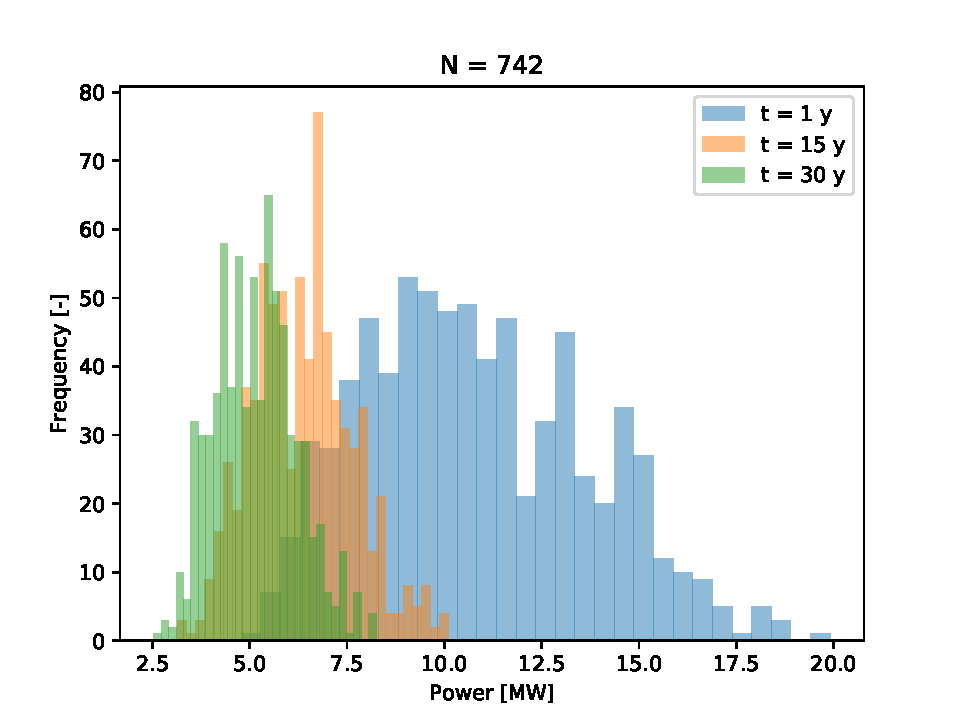
\includegraphics[width=0.5\textwidth]{power_histogram.pdf}
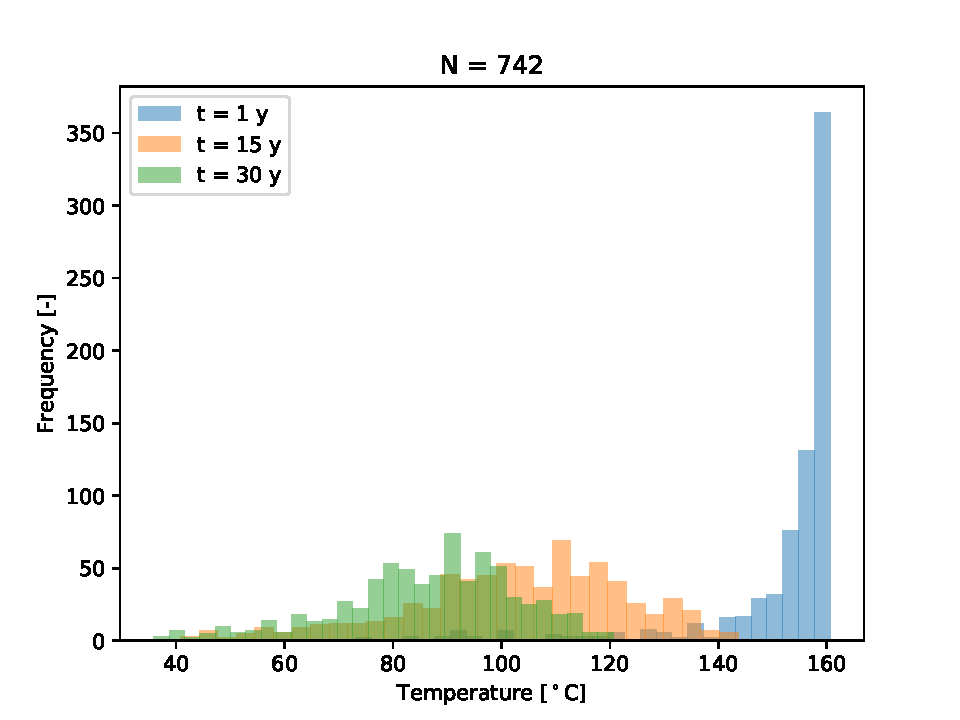
\includegraphics[width=0.5\textwidth]{temp_histogram.pdf}
\caption{Histogram of the output temperature and power in 1,15, and 30 years of operation with the stimulated fractures.}
\end{figure}

\section{Conclusions}
We have developed the HM model for the hydraulic stimulation and the TH model for the heat transfer using consistently the continuum-fracture approach. Although the model is conceptually simple neglecting important thermal effect and contact conditions during the stimulation yet it is capable to reproduce significant effect of the fracture stimulation on the output power and temperature compared to the reference case without stimulation. 

We have shown, that the uncertainty of the power due to fracture dispersion is relatively high in the comparison to the power increase caused by the stimulation. It may indicate relatively high probability
that the stimulation may not result in sufficiently high power for the long term production phase. Further research may investigate if the multiple stimulations can deal with such cases. 







\section*{Acknowledgement}
\begin{itemize}
    \item[a)] RINGEN:
    The research was supported by the Czech Ministry of Education, Youth and Sports under the project No. LM2015084.
 
    \item[b)] RINGEN+:
    The resrarch was supported by the project No. CZ.02.1.01/0.0/0.0/16\_013/0001792, co-funded by the EU Operational Programme ``Research, Development and Education''.
\end{itemize}

\bibliographystyle{dinat}
\bibliography{references.bib}

% \begin{thebibliography}{9}

% \bibitem{brace-et-al} W. F. Brace,  J. B. Walsh, W. T. Grango.  Permeability of Granite Under High Pressure, J. Geophys. Res. 73(6):2225--2236, 1968.

% \bibitem{capova} L. Čápová. Specification of the geothermic model in the environs of several selected boreholes. Diploma thesis, Charles University in Prague, 2013.

% \bibitem{intera} INTERA Environmental Consultants, Inc. Porosity, Permeability,  and Their  Relationship  in  
% Granite,  Basalt, and Tuff. Accession  DE83-011519, NTIS, Springfield, Virginia, 1983.

% \bibitem{martin-jaffre-roberts} V. Martin, J. Jaffré, J. E. Roberts. Modeling fractures and barriers as interfaces for flow in porous media. SIAM Journal on Scientific Computing 26(5):1667--1691, 2005.

% \bibitem{sperl-trckova} J. Šperl, J. Trčková. Permeability and porosity of rocks and their relationship based on laboratory testing. Acta Geodyn. Geomater. 5(149):41--47, 2008.

% \bibitem{ljunggren} C. Ljunggren, O. Stephansson, O. Alm, H. Hakami, U. Mattila. Mechanical properties of granitic rocks from Gide\aa, Sweden. Technical Report 85-06, SKB, 1985.

% \bibitem{zisman} W. A. Zisman. Compressibility and anisotropy of rocks at and near the Earth's surface. Proceedings of the National Academy of Sciences of the United States of America, 19(7):666--679, 1933.

% \end{thebibliography}

\end{document}
